\documentclass[a4paper]{article}
\usepackage[T1]{fontenc}
\usepackage[utf8]{inputenc}
\usepackage[english]{babel}

\usepackage{amsmath}
\usepackage{amssymb}

\usepackage{a4wide}

\usepackage{dsfont}
\usepackage{lmodern}

\usepackage{graphicx}

\title{\textbf{Assignment 1} \\ \small Statistical Methods for Machine Learning }
\author{\textbf{Group members}\\
        Ásbjørn Viderø Jøkladal\\
        Martin Holm Cservenka\\
        Tue Haulund}
\date{17\textsuperscript{th} of February, 2015}		

%=======================================================================
\begin{document}
\maketitle
\tableofcontents
\newpage
%=======================================================================

\section{Probability and Parameter Estimation}
\subsection{Univariate Gaussian Distributions}
Figure~\ref{fig:distributions} shows the 1-dimensional Gaussian density function for the parameter values $(\mu, \sigma) = (-1, 1), (0, 2) \text{ and } (2, 3)$.

\begin{figure}[ht]
  \centering
  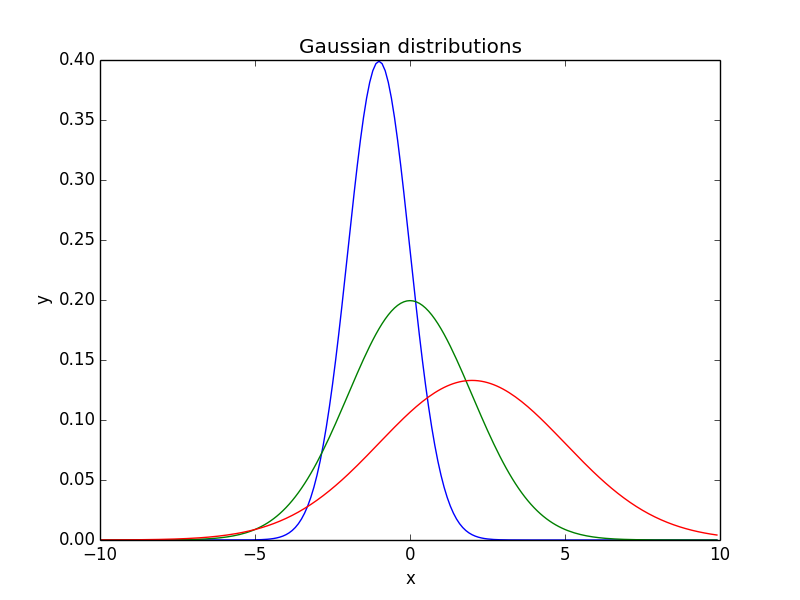
\includegraphics[width=.8\linewidth]{figures/distributions.png}
  \caption{Gaussian density function for the three sets of parameters.}
  \label{fig:distributions}
\end{figure}

\subsection{Sampling from a Multivariate Gaussian Distribution}
Figure~\ref{fig:samples} shows a plot of the generated data set.

\begin{figure}[ht]
  \centering
  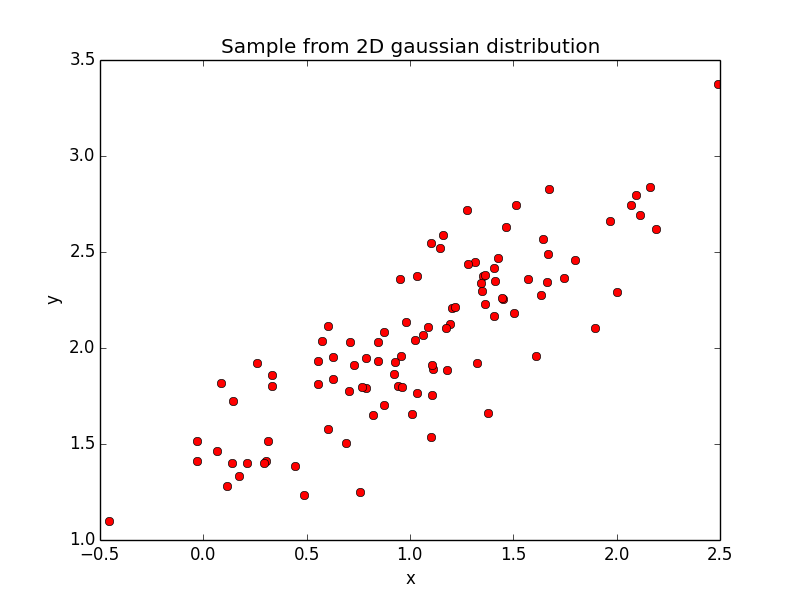
\includegraphics[width=.8\linewidth]{figures/samples.png}
  \caption{Plot of the generated data set.}
  \label{fig:samples}
\end{figure}

\subsection{Means}
Figure~\ref{fig:samples_with_mean} shows the sample mean and the distribution mean together with the data set.

\begin{figure}[ht]
  \centering
  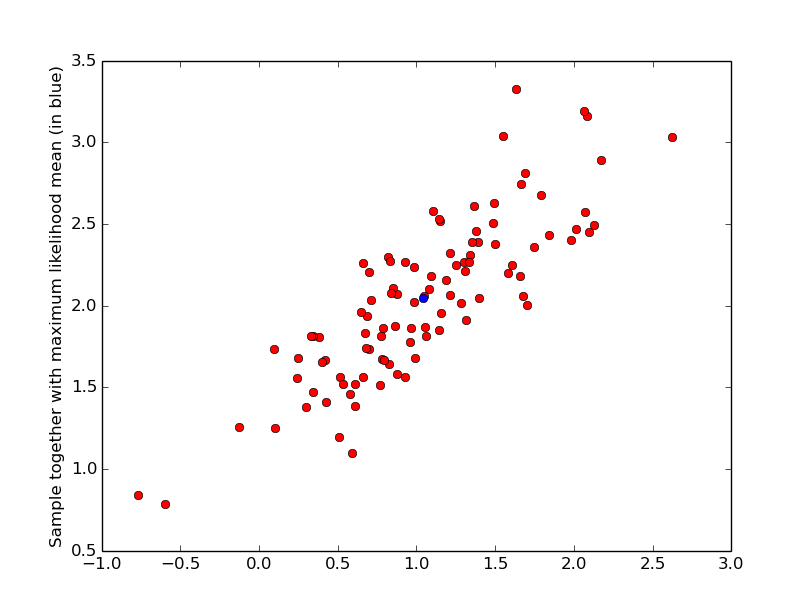
\includegraphics[width=.8\linewidth]{figures/samples_with_mean.png}
  \caption{Plot of the sample mean and the distribution mean together with the data set.}
  \label{fig:samples_with_mean}
\end{figure}

\subsection{Covariance: The Geometry of Multivariate Gaussian Distributions}
Figure~\ref{fig:samples_with_eigenvectors} shows the scaled and translated eigenvectors plotted on top of the sampled data set.

\begin{figure}[ht]
  \centering
  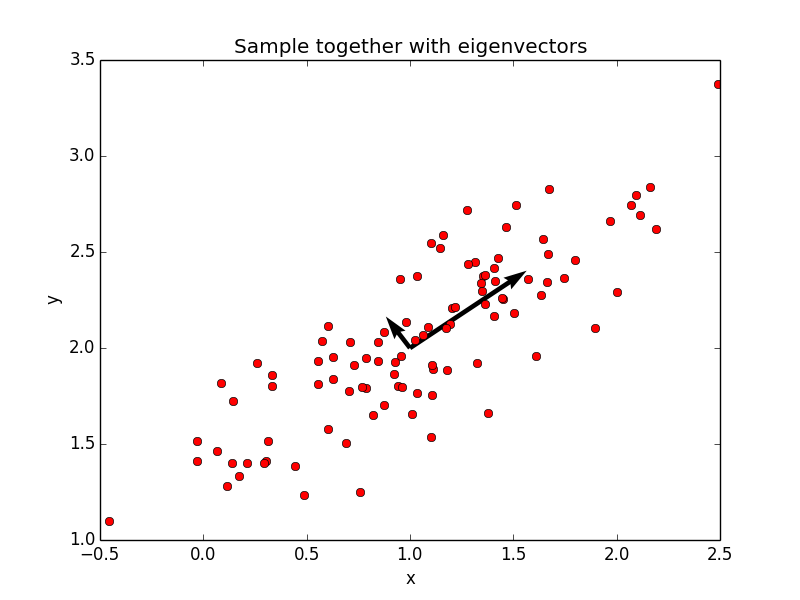
\includegraphics[width=.8\linewidth]{figures/samples_with_eigenvectors.png}
  \caption{Plot of the scaled and translated eigenvectors together with the data set.}
  \label{fig:samples_with_eigenvectors}
\end{figure}

Figure~\ref{fig:samples_rotated} shows samples from the rotated distributions for 30, 60 and 90 degree rotations.

\begin{figure}[ht]
  \centering
  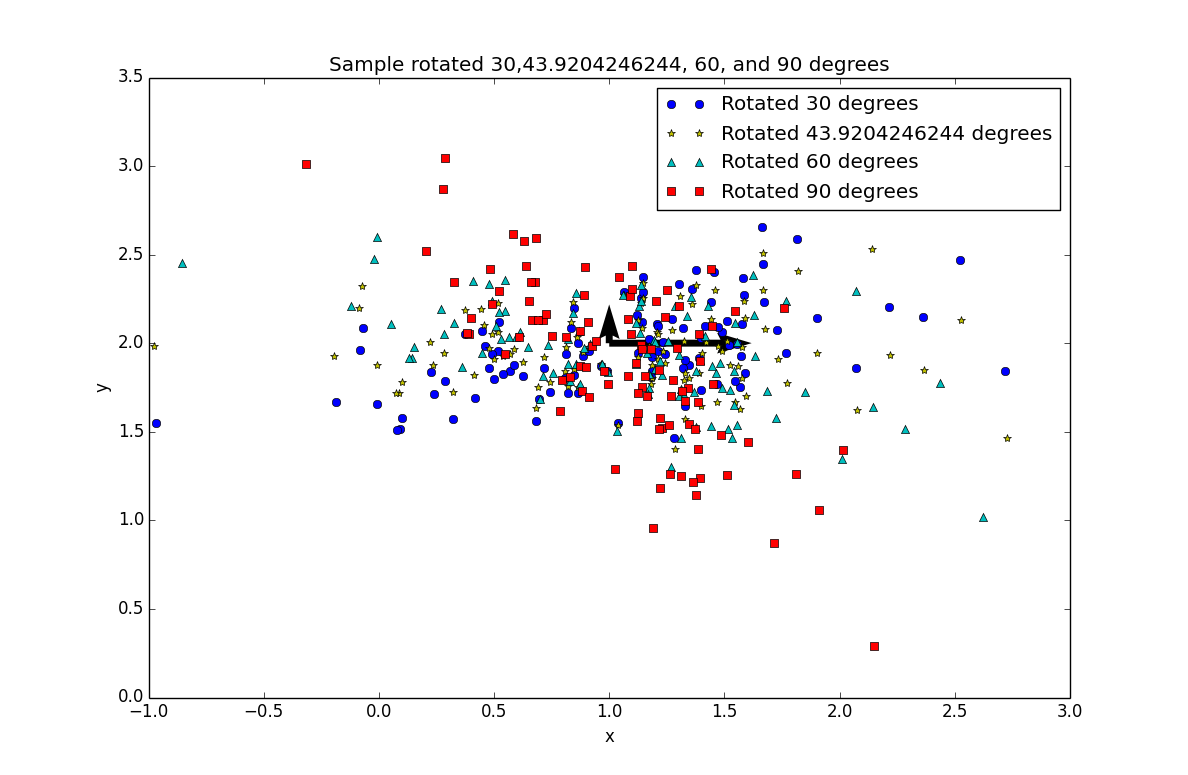
\includegraphics[width=.8\linewidth]{figures/samples_rotated.png}
  \caption{Samples from the rotated distributions.}
  \label{fig:samples_rotated}
\end{figure}

\section{Classification}

\subsection{Nearest Neighbor}

\subsection{Hyperparameter Selection using Cross-validation}

\subsection{Data Normalization}



\end{document}
